\documentclass{article}

\usepackage[a4paper, top=2cm, bottom=3cm]{geometry}

\usepackage[ngerman]{babel}
\usepackage{csquotes}

\usepackage{booktabs}
\usepackage{mathtools}
\usepackage{amssymb}
\usepackage{enumitem}
\usepackage{amsmath}

\usepackage{hyperref}

\usepackage{graphicx}
\usepackage{wrapfig}

\usepackage{pgfplots}

\usepackage{siunitx}

\usepackage{biblatex}
\DefineBibliographyStrings{ngerman}{
  urlseen = {Abruf vom}
}
\addbibresource{quellen.bib}

\newcommand{\proofeq}{\overset{!}{=}}
\newcommand{\proofeqv}{\overset{!}{\Leftrightarrow}}
\newcommand{\equivalent}{\overset{\scriptscriptstyle\wedge}{=}}
\DeclarePairedDelimiter\ceil{\lceil}{\rceil}
\DeclarePairedDelimiter\floor{\lfloor}{\rfloor}

\date{7.03.2022}
\title{Physikalisches Grundpraktikum Teil I \\ (Mechanik und Thermodynamik) \\ Versuch 2 Drehbewegung}
\author{Finn Bietz, Finn Wagner}

\begin{document}
	
	\maketitle

	TODO: GIMP Bild machen

	\section{Versuchsziel und Versuchsmethode}
			In diesem Experiment soll das Trägheitsmoment eines Kreisels über drei verschiedene Methoden bestimmt werden.
			TODO: Was ist ein Trägheitsmoment?
			TODO: Formeln
			TODO: Noch was aus der Aufgabenstellung abschreiben?

	\section{Trägheitsmoment über die Winkelbeschleunigung}

		\subsection{Grundlagen}

		\subsection{Durchführung}
		\begin{enumerate}
			\item Masse des Gewichts \(m\) messen.
			\item Messen des Radius der Schnuraufwicklung mit dem Messschieber

			\item Aufwickenln des Fadens und anhängen des Gewichts an die Kreisscheibe.
			\item Zeitmessung für Umdrehungen mit \enquote{Runden} Knopf von Smarthphone Stoppuhr

		\end{enumerate}

		Durch Anhängen eines Gew

		\subsection{Ergebnisse}
		TODO: Messergebnisse Abschreiben
		Mit Hilfer der Waage wurde die Masse des kleinen Gewichts \(m\) auf \(\SI{99}{\gram}\) bestimmt.
		Die benutzte Waage hat eine Genauigkeit von einem Gramm.
		Die Schnuraufwicklung hat den Radius \(r = \SI{4.93}{\centimetre}\). Die dazu verwendete Schieblehre
		hat eine Genauigkeit von \(\SI{0.05}{\millimetre}\) 

		\begin{tabular*}{c c c c c c}
			Anzahl Umdrehungen & 1 & 2 & 3 & 4 & 5 \\
			Verstrichen Zeit & \(\SI{4.89}{\second}\) & \(\SI{2.14}{\second}\) &  \(\SI{1.67}{\second}\) & \(\SI{1.33}{\second}\) & \(\SI{1.21}{\second}\) \\
		\end{tabular*}
		Für die Messungen wurde eine Handystoppuhr verwendet. Der Winkel wurde mit dem Auge geschätzt. Messwerte aus\ref{fig:Messwerte1}.

		\subsection{Fehlerrechnung}
		Maximaler Fehler, aus m, r, S

		\subsection{Auswertung}
			\subsubsection{Formeln}
				Durch anhängen des Gewichts mit der Masse \(m\) auf den aufgewickelten Faden erzeugt man ein Drehmoment \(M = mgr\) wodurch der Kreisel eine konstante Winkelbeschleunigung
				\begin{equation}
					M = I \alpha = I \frac{d\omega}{dt}
				\end{equation}
				erfährt.
				Zwischen dem Winkel und der Winkelbeschleunigung besteht die Beziehung (wenn der Kreisel mit Winkelgeschwindigkeit und Winkel 0 beginnt \(\omega = \phi = 0\))
				\begin{equation}
					\phi = \frac{1}{2} \alpha t^2
				\end{equation}
				Setzen wir die beiden Formeln TODO:Refs in einander ein, so ergibt Schieblehre
				\begin{equation}
					I = \frac{M}{\alpha} = \frac{Mt^2}{2\phi}
				\end{equation}

			TODO: Einsetzen

		\subsection{Endergebnis}
		TODO: ?

	\section{Trägheitsmoment über die Schwingungsdauer einer Pendelbewegung}

	\section{Trägheitsmoment über eine Präzessionsbewegung}

	\section{Fazit}
	TODO: Welcher Versuch ist am Besten geignet, am einfachsten, am genausten, etc... um das Trägheitsmoment zu bestimmen.
	Vergleich der Ergebnisse
    Hoffentlich ähnliche Ergebnisse.
    Diskutiere z.B Reibungseffekte, Kleinwinkelnäherung, etc.
    Fazit beste Methode, z.B. kleinester Fehler, Durchführung am wenigsten Aufpassen.


	\printbibliography[title={Quellen}]

	\begin{figure}[!h]\label{fig:Messwerte1}
		\centering
		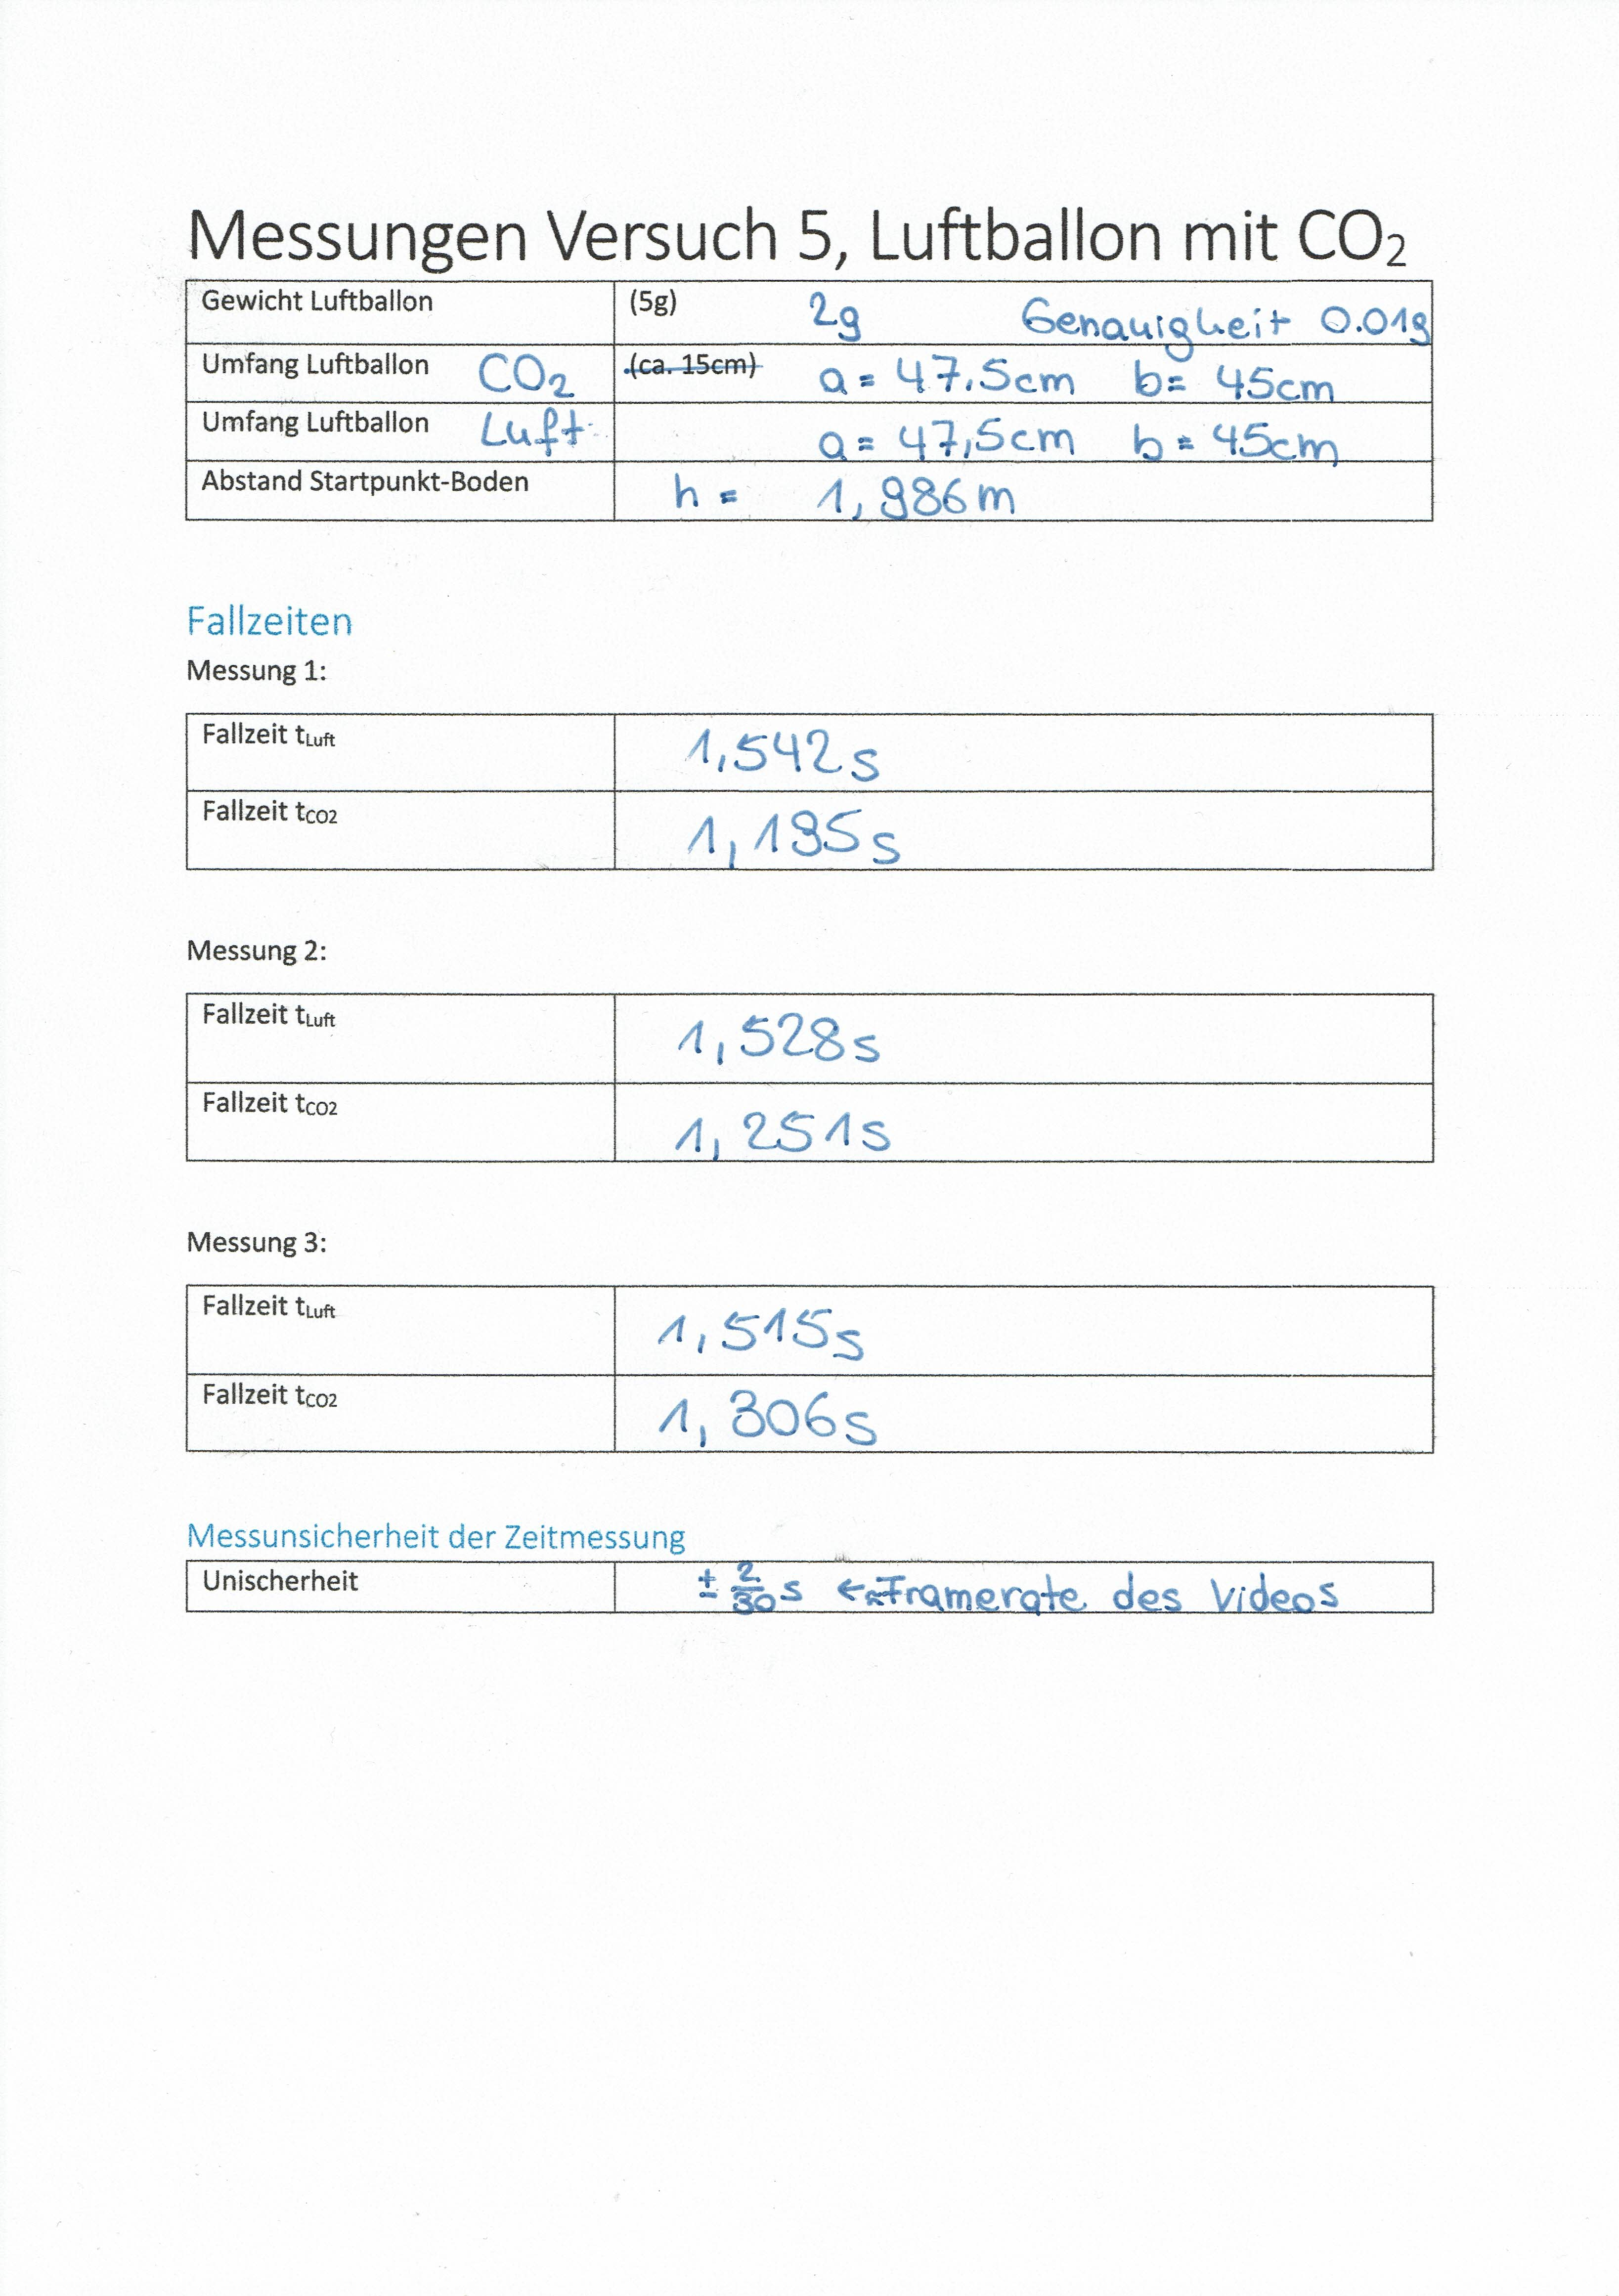
\includegraphics[height=14cm]{messwerte.jpg}
		\caption{Messwerte der drei Versuchsdurchführungen}
	\end{figure}

	\begin{figure}[!h]\label{fig:Messwerte2}
		\centering
		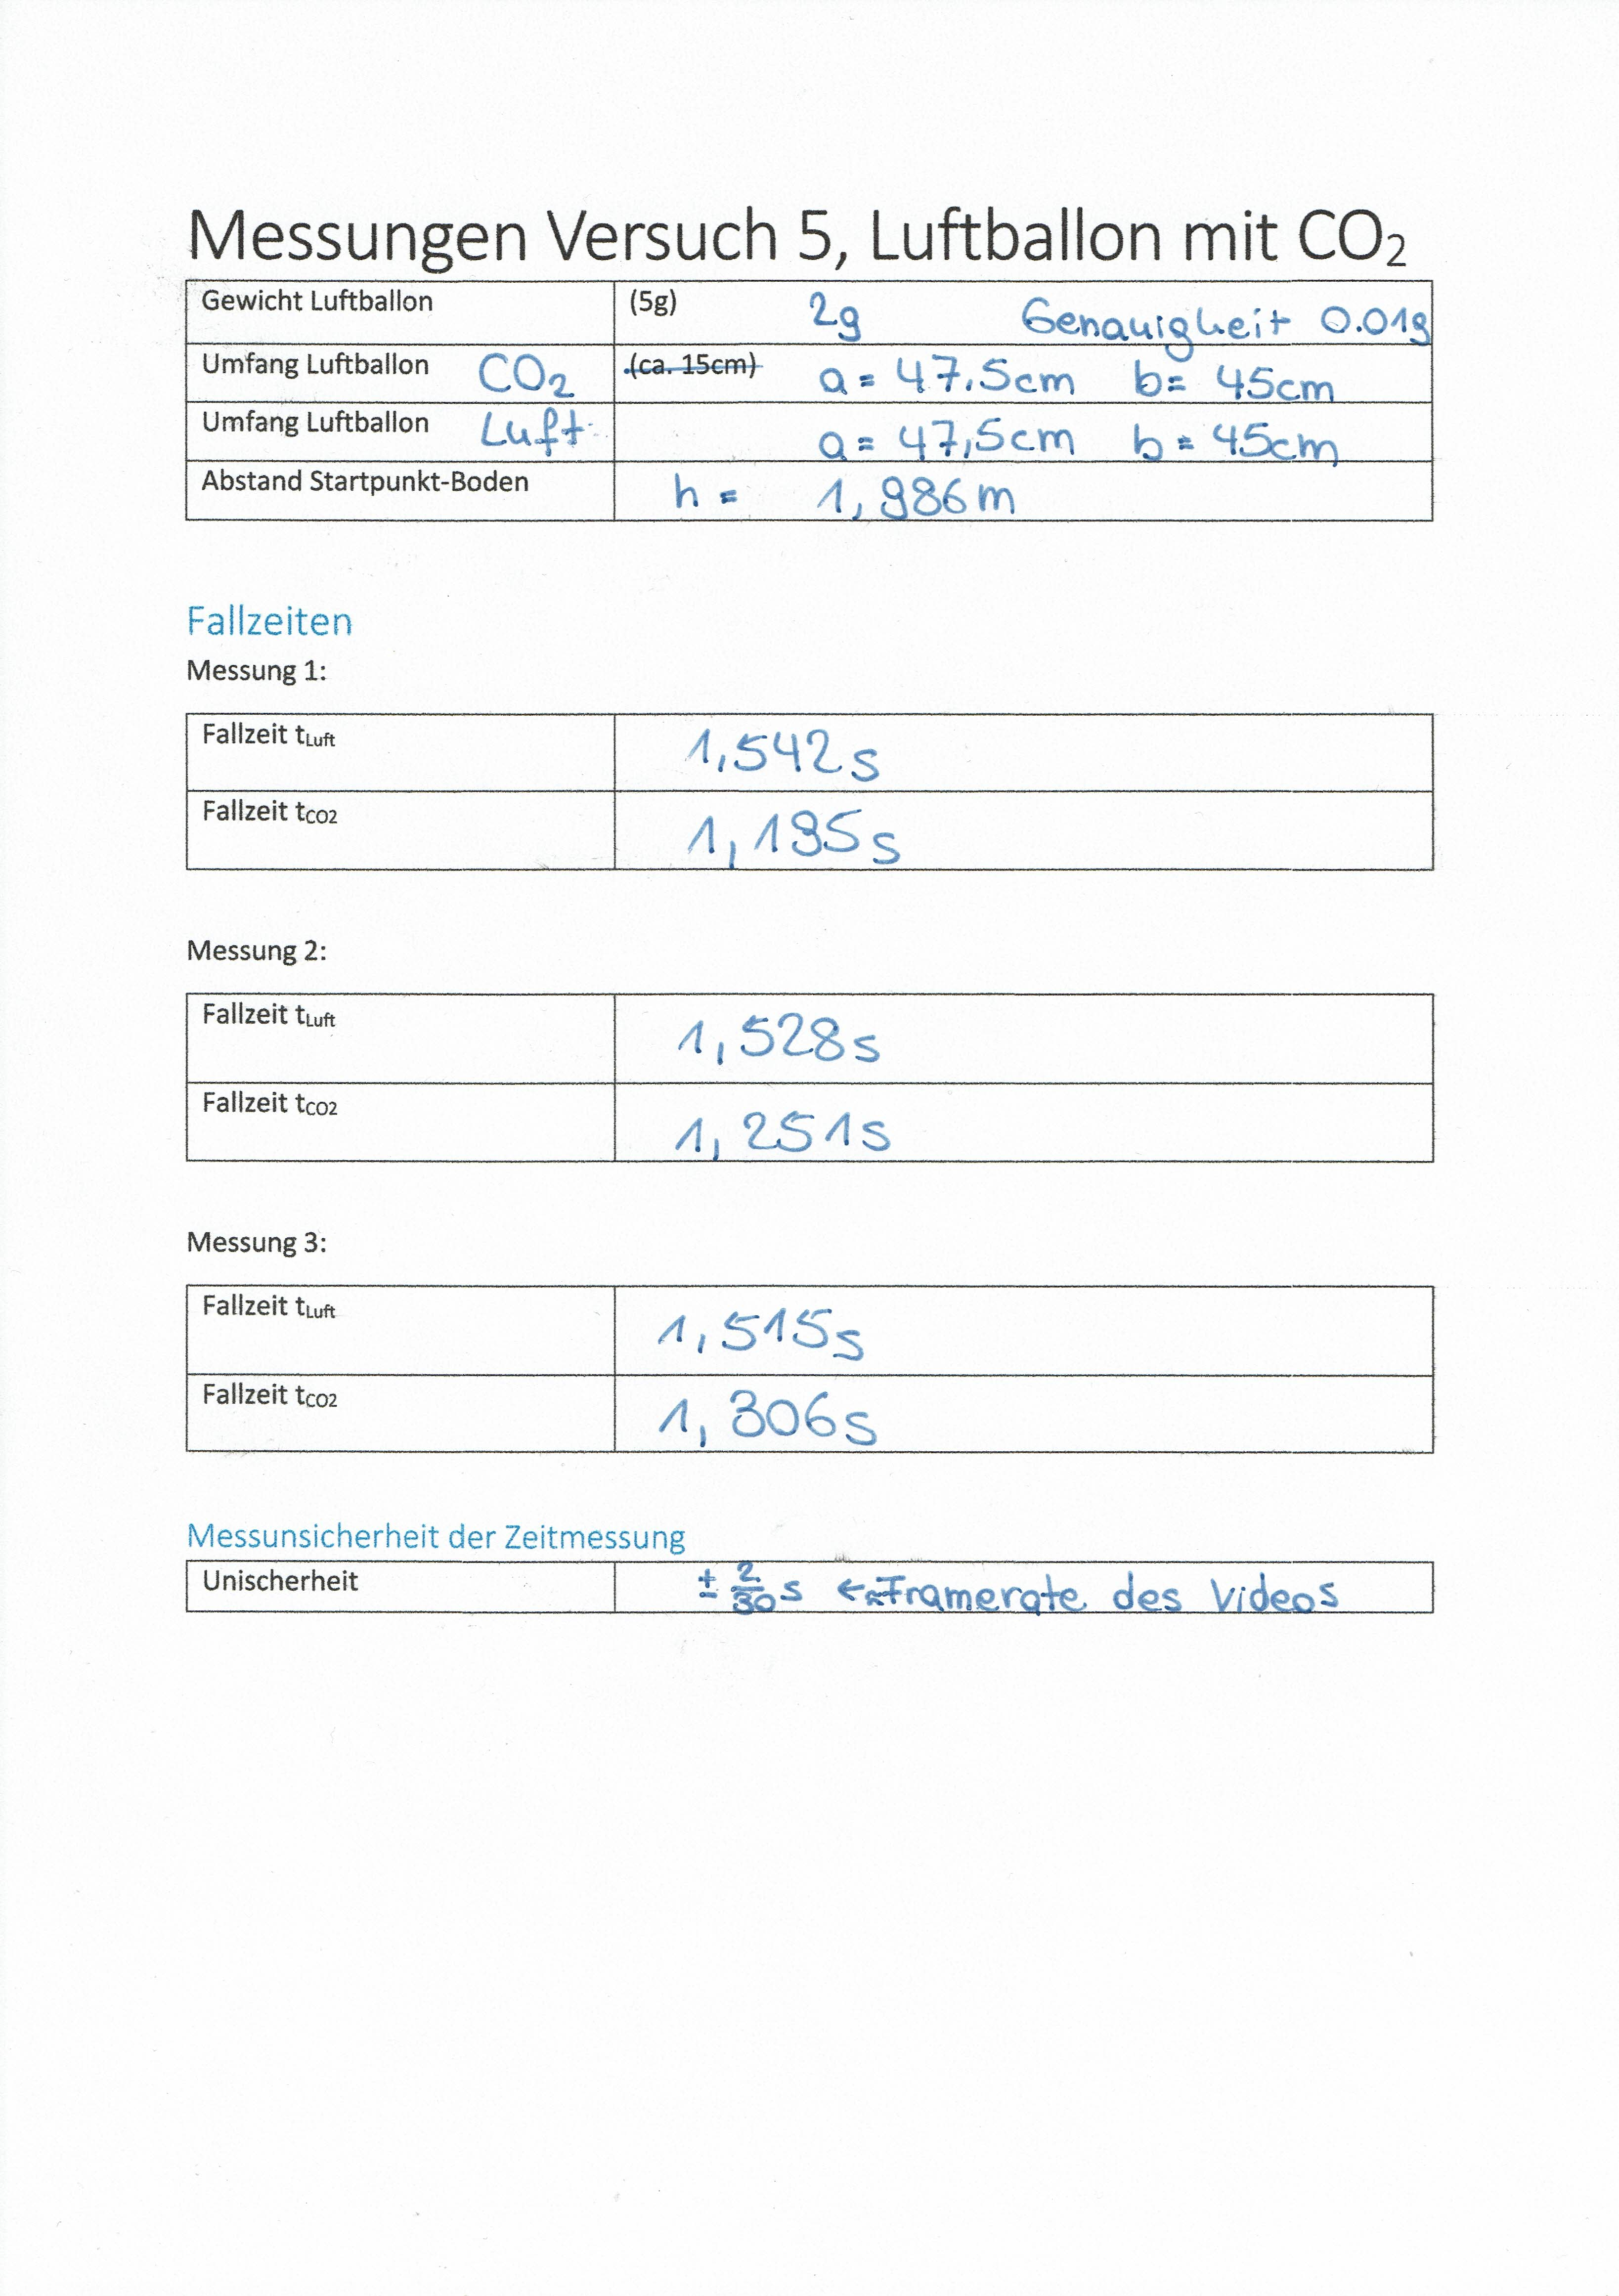
\includegraphics[height=14cm]{messwerte.jpg}
		\caption{Messwerte der drei Versuchsdurchführungen}
	\end{figure}

\end{document}